\chapterimage{Week3Clarifier1.jpg} % Chapter heading image

\chapter{Liquid Treatment Part I}

\section{Collection}\index{Collection}	
The collection system resembles a tree that branches out from the treatment plant to collect the wastewater from individual sources.

\subsection{Wastewater Collection Piping}\index{Wastewater Collection Piping}	
	\begin{itemize}
		\item A \hl{lateral} is the piping that connects the public sewer to the building. 
		\item Laterals flow into larger lines called \hl{mains}.
		\item Mains carry the flow into the largest lines in the system, called \hl{trunk lines}. 
		\item A trunk line is the pipe that brings water into the treatment plant.
	\end{itemize}
\subsection{Sanitary Sewer Systems}\index{Sanitary Sewer Systems}

Sanitary sewer systems collect and convey wastewater from residential, commercial and industrial sources to a centralized wastewater treatment facility for treatment. 

\subsubsection{Storm-water systems}\index{Storm-water systems}

Storm-water systems are designed solely for the conveyance of storm-waters waters directly to streams, rivers, lakes, or the ocean.
 
\subsubsection{Combined sewer systems}\index{Combined sewer systems}
\begin{itemize}
\item Combined sewer systems collect and convey sanitary sewage and urban runoff in a common piping system.
\item Combined sewers could potentially cause serious water pollution problems during combined sewer overflow (CSO) events when wet weather flows exceed the sewage treatment plant capacity.
	\end{itemize}
\begin{center}
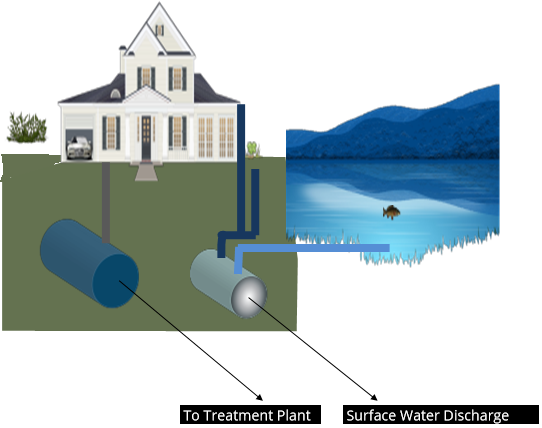
\includegraphics[scale=0.45]{SeperatedSystem1} \hspace{1 cm} 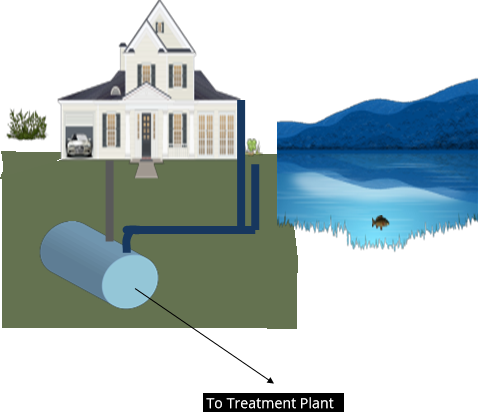
\includegraphics[scale=0.45]{CombinedSystem1}
\end{center}
			\hspace{2.6cm} Separated System \hspace{3.2cm} \parbox{\textwidth}{Combined System}\\

\subsection{Collections Systems Basics}\index{Collections Systems Basics}
	\begin{itemize}
\item The primary type of a collection system is a \hl{gravity system}. A gravity system is so named because the wastewater flows down gradient in the sewer, driven by forces of gravity. 
\item The collection system includes the gravity sewers, force mains, manholes, pumping equipment, and other facilities that collect and convey the water to a wastewater treatment plant. 
\item Sewers are generally laid at a minimum slope to ensure open channel flow through the pipe at a \hl{minimum velocity of 2.0 feet per second}. The minimum velocity is required to ensure that solids do not settle out in the sewer.  
\item When the sewer lines reach a certain depth, the flow must be lifted back through a lift or pump station.  
\item \hl{Lift stations} are built whenever wastewater must be pumped to a higher altitude, whether it's to lift water up so that it can gravity flow or to pump it over a rise or hill.  
\item The discharge from the pump station may be to another gravity sewer at that location or through a pressurized force main. 
\item Key elements of lift stations include a wastewater receiving well (wet-well), pumps and piping with associated valves.
\item The size of the wet well affects the operating of the station. If a wet well is too small, excessive starting and stopping of the pump motors will occur, resulting in premature failure. If the wet well is too large, solids will tend to settle on the bottom, blocking the pump suction line and leading to the generation of hydrogen sulfide and methane.
\item The dry well is the portion of the dry well/wet well pumping station that houses the necessary equipment required to pump the wastewater. The dry well is so named because it is isolated from the incoming wastewater.
\item Centrifugal pumps are the most common type of pump found in wastewater pumping stations. 
\item In the USA, wastewater generated in a typical home is about 70 gal/day/person
\end{itemize}


\section{Preliminary Treatment}\index{Preliminary Treatment}

			\begin{itemize}
				\item The objective of preliminary treatment is to remove coarse solids and other large materials often found in raw wastewater
				\item Removal of these materials is necessary to enhance the operation and maintenance of subsequent treatment units\\
				\item Preliminary treatment operations typically include a combination of the following processes:
					\begin{itemize}
						\item Screening
						\item Grinding or shredding
						\item Flow measurement
						\item Grit removal
						\item Pre-aeration
						\item Flow equalization
					\end{itemize}
			\end{itemize}

				
		\subsection{Process Elements of Preliminary Treatment}\index{Process Elements of Preliminary Treatment}	
			
		\subsubsection{Screening}\index{Screening}
					\begin{itemize}
						\item Screening is typically the first unit in a preliminary treatment
						\item Screening allows for the capture of coarse solids as pieces of cloths garbage so as to protect pumps and other units from clogging. 
						\item Screens may consist of vertical or inclined bars (bar racks or bar screens), wire mesh or perforated plates having either circular or rectangular openings. 
						\item Screens remove the large, entrained, suspended or floating solids such as pieces of wood, cloth, paper, plastics, garbage, etc.
						\item Debris collected on the screen can be cleaned manually or automatically using chain driven rakes 
						\item The retained material at screens - screenings, is collected and hauled to landfill for disposal
						\item The quantity of screenings removed varies by location and is a function of the clear opening of the screen.
						\item Barmuinitors combine the function of a screen and a grinder.  The ground material is returned to the wastewater flow for removal during primary treatment.
					\end{itemize}

\begin{figure}
\begin{center}
    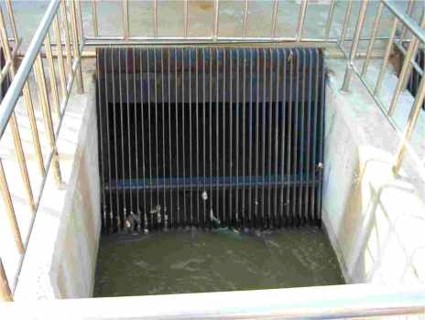
\includegraphics[width=0.7\linewidth]{Barscreen}\\

Barscreen - No rakes
\end{center}
  \end{figure}
  

		\subsubsection{Grinding and Shredding}\index{Grinding and Shredding}

					\begin{itemize}
\begin{minipage}{\textwidth}	\item Comminutor(Grinder) consist of fixed, rotating or oscillating teeth or blades, acting together to reduce the solids to a size which will pass through fixed or rotating screens grind rags into small chunks
\item The comminutors are installed in wastewater channel and they grind the larger solids without actually removing them from the wastewater.  These devices may be installed before the screens or as a combination of screen and cutters (barmunitors).
					\end{minipage}	
					\end{itemize}
					\begin{minipage}{\textwidth}
					\begin{center}
      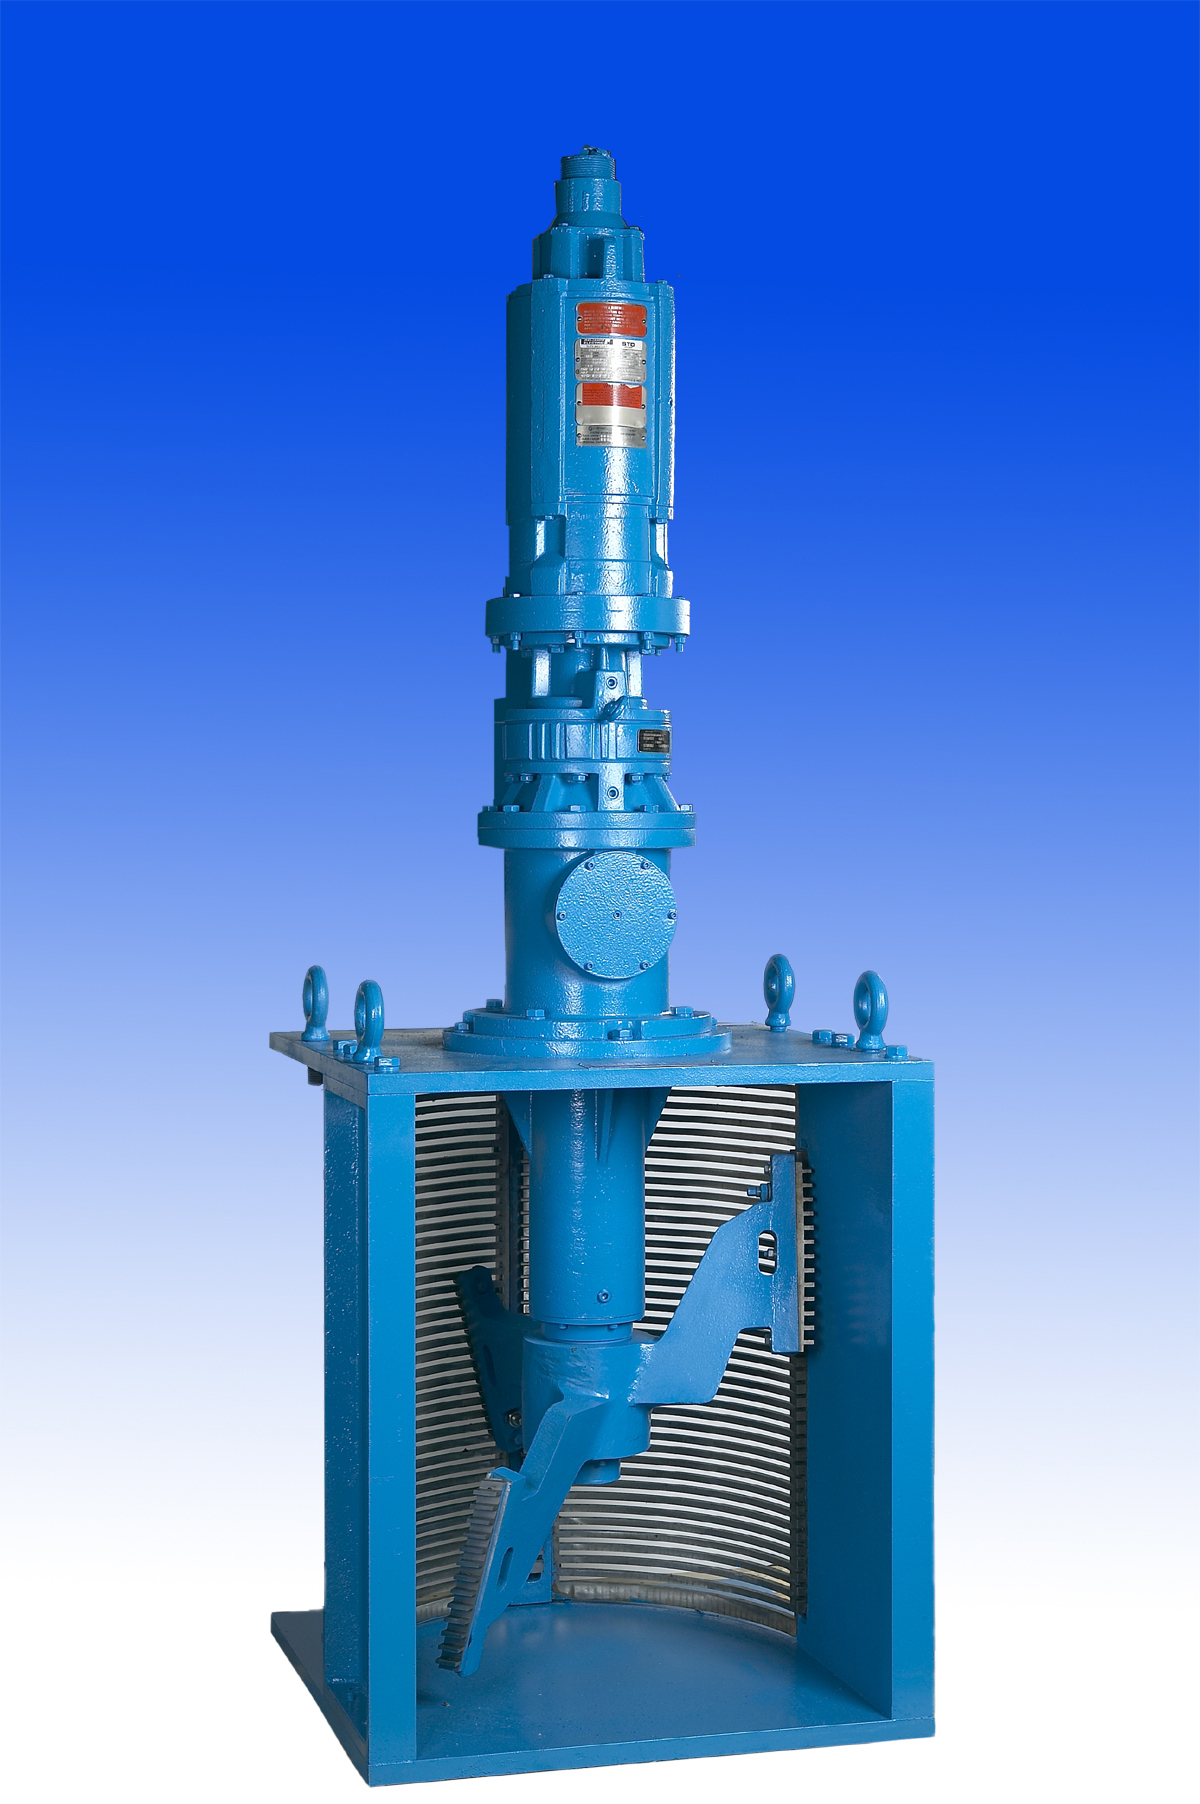
\includegraphics[width=0.3\linewidth, height=70mm]{Comminutor}\\
      Comminutor\\
\end{center}
    \end{minipage}
  
		\subsubsection{Flow Measurement}\index{Flow Measurement}
					\begin{itemize}
						\item Wastewater flow to a treatment plant is not constant but varies in a diurnal (daily) pattern reflecting domestic water use activity.
						\item Continuous flow measurement is necessary in order to monitor diurnal variations in flow which may affect treatment plant efficiency.\\
						\item Devices used for flow measurement as part of the preliminary treatment can be placed in a channel or in a pipe.
					\end{itemize}


		\subsection{Grit Removal}\index{Grit Removal}
						\begin{itemize}
							\item Grit includes sand, gravel, cinder, eggshells, bone chips, seeds, coffee grounds, and large organic particles, such as food waste.
							\item Purpose of Grit removal:
								\begin{itemize} 
									\item to protect mechanical equipment from abrasion and abnormal wear 
									\item to reduce clogging caused by deposition of grit particles in pipes and channels, and 
				\item to prevent loading the treatment plant with inert matter that might interfere with the operation of treatment units such as anaerobic digester and aeration tanks.
			\end{itemize}
		\item Removal of organic material along with the grit is undesirable for two reasons:
			\begin{enumerate}
				\item It causes odor issues, and 
				\item Organic matter is a potential source of energy (digester gas)
			\end{enumerate}
		\item Grit Disposal: Grit removed is typically landfilled.
		\item Grit Volume:  The volume of grit collected measured in ft$^3$/MG.
		\item The rate of grit collection can range from 0.5 ft$^3$/MG to 30 ft$^3$/MG.
		\item Wastewater plants having a combined collection system must deal with much larger volumes of grit.
\end{itemize}

\begin{figure}[h!]
  \centering
  \begin{subfigure}[b]{0.46\linewidth}
    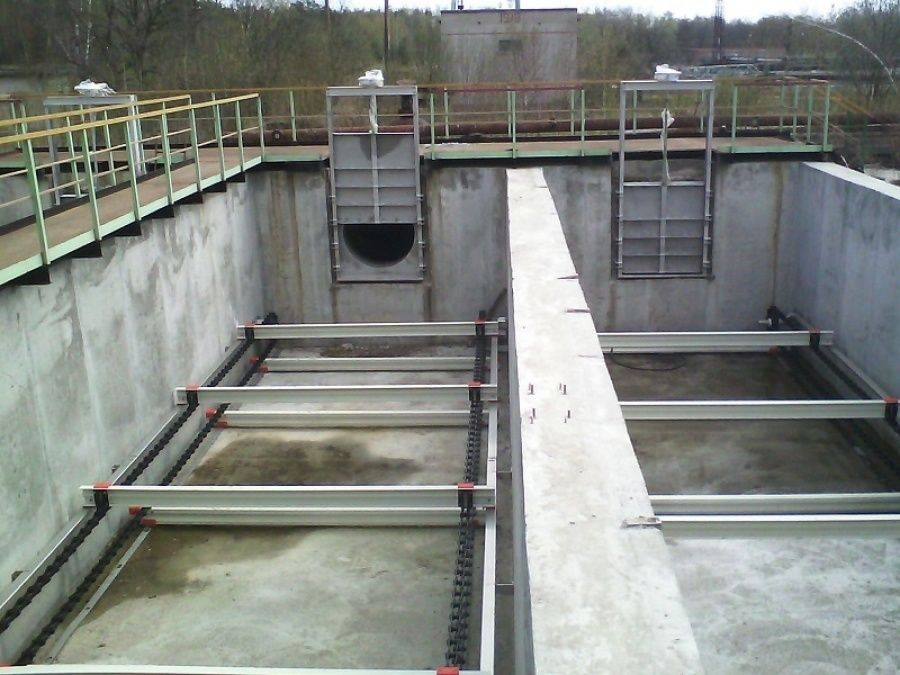
\includegraphics[width=0.8\linewidth]{HorizontalGritChamber}
    \caption{Horizontal grit chamber}
  \end{subfigure}
  \hspace{0.2cm}
  \begin{subfigure}[b]{0.5\linewidth}
    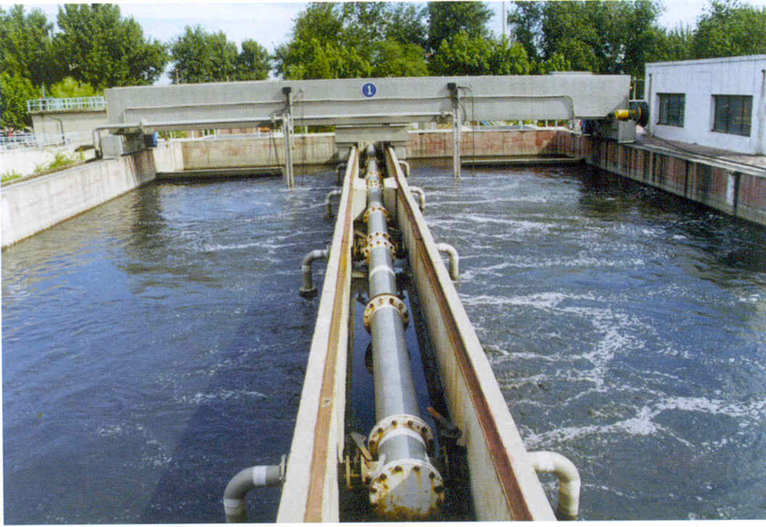
\includegraphics[width=0.8\linewidth]{AeratedGritChamber}
    \caption{Aerated grit chamber}
  \end{subfigure}
\end{figure} 					

\begin{figure}[h!]
  \centering
  \begin{subfigure}[b]{0.47\linewidth}
    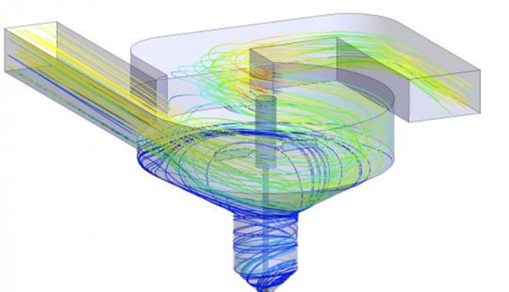
\includegraphics[width=0.8\linewidth]{VortexGritChamber1}
    \caption{Vortex grit chamber design}
  \end{subfigure}
  \hspace{0.2cm}
  \begin{subfigure}[b]{0.43\linewidth}
    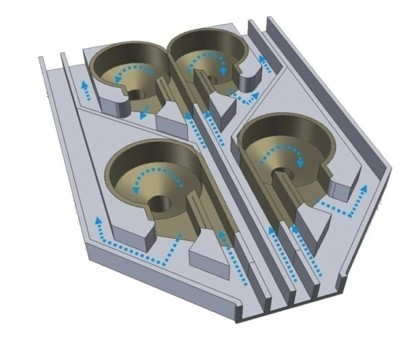
\includegraphics[width=0.8\linewidth]{VortexGritChamber}
    \caption{Vortex grit chamber installed}
  \end{subfigure}
\end{figure} 

\subsection{Pre-aeration}\index{Pre-aeration}	
	\begin{itemize}
		\item Pre-aeration of the wastewater as part of the preliminary treatment may be provided as a separate process or increased detention time in an aerated grit chamber.
		\item Pre-aeration provides the follwoing benefits:
			\begin{itemize}
				\item freshens up wastewater by dissolving oxygen thereby reducing the wastewater septicity
				\item reduction of septicity allows for better settling - solids and BOD removal, in the following primary treatment process
				\item promotes grease separation which facilitates its removal during primary treatment
			\end{itemize}
	\end{itemize}
\subsection{Flow Equalization}\index{Flow Equalization}	

	\begin{itemize}
		\item Flow equalization involves storing a portion of peak flows for release during low-flow periods
		\item It prevents surges and allows for the operation of processes at design flows thus allowing for optimal physical, biological and chemical processes to take place.
		\item It results in saving capital costs as the processes may be built with a treatment capacity which is less than the peak flows
	\end{itemize}

\section{Primary Treatment}\index{Primary Treatment}	

\begin{itemize}
\item Synonyms:  primary treatment basin, primary clarifier, sedimentation basin, primaries, clarifier

	
		\item Primary treatment is after preliminary treatment and 				before secondary treatment
		\item Its two main objectives are: 
			\begin{itemize}
				\item Remove settleable solids
				\item Remove floatable solids
			\end{itemize}
		\item This is a physical process which relies on the physical 			properties - how heavy or light the suspended solids particles 		are to effect its separation
		\item Provides quiescent conditions for the influent 					wastewater for the heavier solids to settle and the lighter 			solids to float
		\item Removes settleable solids and floatables
		\item Settled solids are removed as sludge from the bottom of 			the clarifier
		\item Floatable solids including oil and grease are also 				removed, as scum from the surface\\
		\item The shape of the primary clarifier is either rectangular 		or circular
	
		\item Effective solids removal in the primary clarifiers will 			reduce the loading on the expensive secondary treatment 				process.
		\item The amount of solids removed during primary treatment 			may be enhanced by chemical addition - ferric or ferrous 				chloride as a coagulant and anionic polymer as the flocculant.  		This is called Chemically Enhanced Primary Treatment (CEPT).
		\begin{center}
				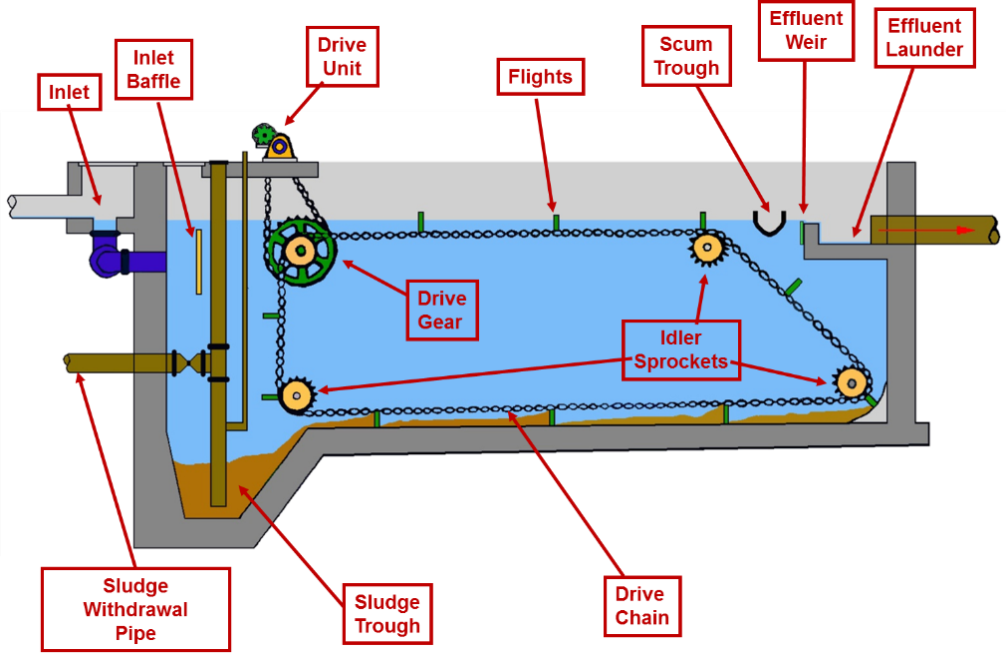
\includegraphics[scale=0.9]{RectangularClarifier}\\
				Cross section of a Rectangular Clarifier\\
				
\includegraphics[scale=0.1]{Blank}\\
				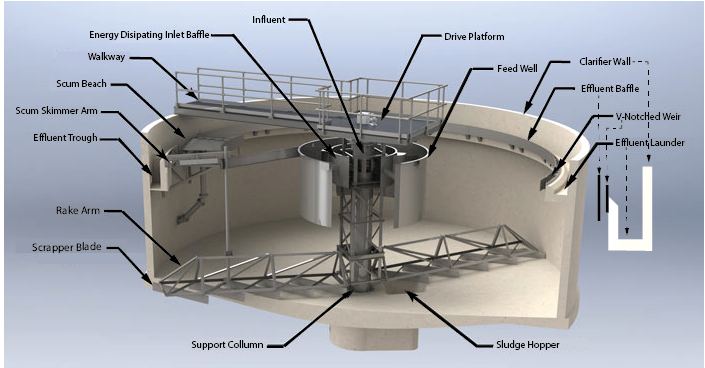
\includegraphics[scale=0.5]{CircularClarifier3}\\
				Cross section of a circular clarifier\\
			\end{center}
				
\includegraphics[scale=0.03]{Blank}\\
\item \textbf{Typical Removal Rates:}\\
\begin{itemize}
\item \hspace{10mm} BOD removal – 25\% to 40\% and about 60\% with CEPT
\item \hspace{10mm} Suspended solids (SS) removal – 40\% to 60\% and about 75\% with CEPT
\item \hspace{10mm} Settleable Solids removal - $>$90\%
\end{itemize}
\end{itemize}



